\documentclass[tikz,border=8pt]{standalone}
% Shared look for every TikZ diagram. Load with % Shared look for every TikZ diagram. Load with % Shared look for every TikZ diagram. Load with \input{../../tools/tikz-style.tex}
\usepackage[T1]{fontenc}
\usepackage{lmodern}
\renewcommand{\sfdefault}{lmr}  % diagrams use the same serif as the text
\usetikzlibrary{arrows.meta, positioning, shapes.geometric, calc, fit, backgrounds}
\definecolor{cblue}{HTML}{4C78A8}
\definecolor{corange}{HTML}{F58518}
\definecolor{cgreen}{HTML}{54A24B}
\definecolor{cred}{HTML}{E45756}
\definecolor{cpurple}{HTML}{B279A2}
\definecolor{cgrey}{HTML}{6B6B6B}
\tikzset{
  every picture/.style={font=\sffamily, line width=1.2pt},
  box/.style={draw=#1, fill=#1!12, rounded corners=4pt, align=center, inner sep=7pt, minimum height=1.1cm},
  box/.default=cgrey,
  arrow/.style={-{Stealth[length=3mm]}, draw=cgrey, line width=1.4pt},
  title/.style={font=\sffamily\bfseries\Large},
  note/.style={font=\sffamily\small, text=cgrey, align=center},
}
\AtBeginDocument{\hyphenpenalty=10000 \exhyphenpenalty=10000}

\usepackage[T1]{fontenc}
\usepackage{lmodern}
\renewcommand{\sfdefault}{lmr}  % diagrams use the same serif as the text
\usetikzlibrary{arrows.meta, positioning, shapes.geometric, calc, fit, backgrounds}
\definecolor{cblue}{HTML}{4C78A8}
\definecolor{corange}{HTML}{F58518}
\definecolor{cgreen}{HTML}{54A24B}
\definecolor{cred}{HTML}{E45756}
\definecolor{cpurple}{HTML}{B279A2}
\definecolor{cgrey}{HTML}{6B6B6B}
\tikzset{
  every picture/.style={font=\sffamily, line width=1.2pt},
  box/.style={draw=#1, fill=#1!12, rounded corners=4pt, align=center, inner sep=7pt, minimum height=1.1cm},
  box/.default=cgrey,
  arrow/.style={-{Stealth[length=3mm]}, draw=cgrey, line width=1.4pt},
  title/.style={font=\sffamily\bfseries\Large},
  note/.style={font=\sffamily\small, text=cgrey, align=center},
}
\AtBeginDocument{\hyphenpenalty=10000 \exhyphenpenalty=10000}

\usepackage[T1]{fontenc}
\usepackage{lmodern}
\renewcommand{\sfdefault}{lmr}  % diagrams use the same serif as the text
\usetikzlibrary{arrows.meta, positioning, shapes.geometric, calc, fit, backgrounds}
\definecolor{cblue}{HTML}{4C78A8}
\definecolor{corange}{HTML}{F58518}
\definecolor{cgreen}{HTML}{54A24B}
\definecolor{cred}{HTML}{E45756}
\definecolor{cpurple}{HTML}{B279A2}
\definecolor{cgrey}{HTML}{6B6B6B}
\tikzset{
  every picture/.style={font=\sffamily, line width=1.2pt},
  box/.style={draw=#1, fill=#1!12, rounded corners=4pt, align=center, inner sep=7pt, minimum height=1.1cm},
  box/.default=cgrey,
  arrow/.style={-{Stealth[length=3mm]}, draw=cgrey, line width=1.4pt},
  title/.style={font=\sffamily\bfseries\Large},
  note/.style={font=\sffamily\small, text=cgrey, align=center},
}
\AtBeginDocument{\hyphenpenalty=10000 \exhyphenpenalty=10000}

\begin{document}
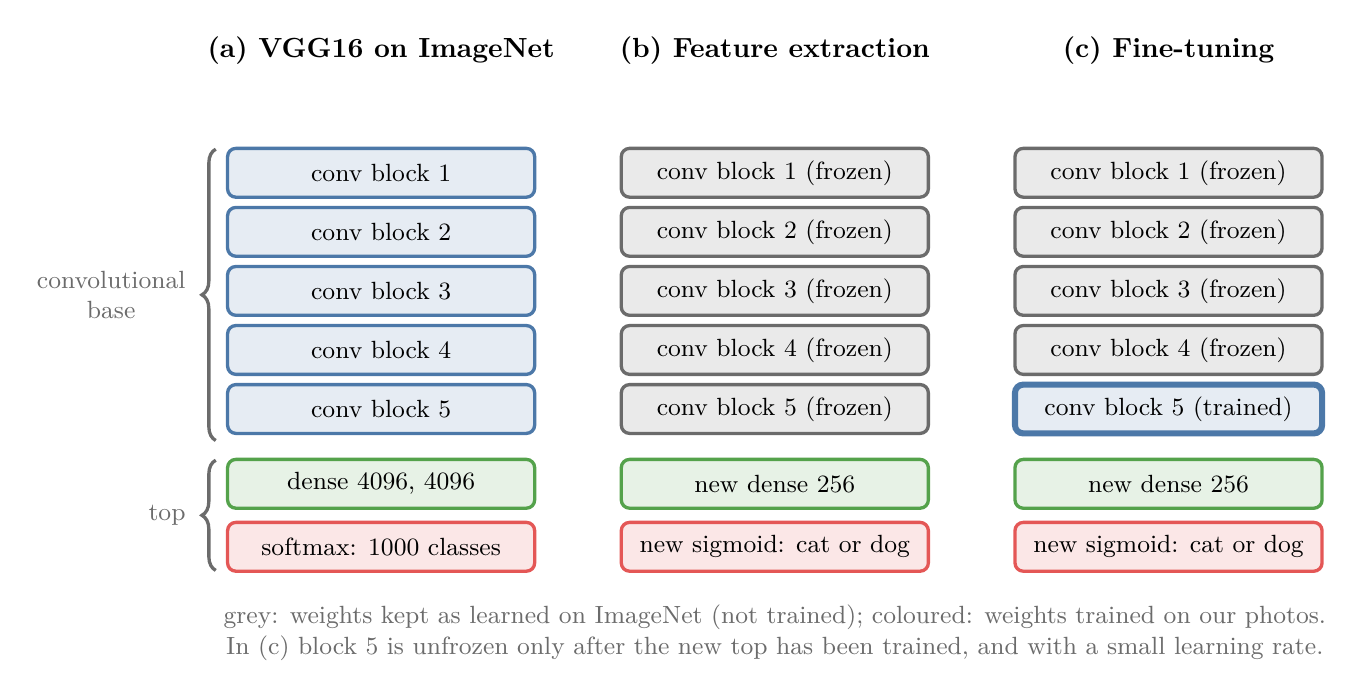
\begin{tikzpicture}[
    blk/.style={draw=#1, fill=#1!14, rounded corners=3pt, minimum width=3.9cm, minimum height=0.62cm, font=\sffamily\small, inner sep=2pt},
    frozen/.style={blk=cgrey, pattern color=cgrey},
    lab/.style={font=\sffamily\small, align=center}]
  % columns: (a) trained on ImageNet, (b) feature extraction, (c) fine-tuning
  \foreach \x/\ttl in {0/{(a) VGG16 on ImageNet}, 5.0/{(b) Feature extraction}, 10.0/{(c) Fine-tuning}} {
    \node[title, font=\sffamily\bfseries] at (\x, 0.9) {\ttl};
  }
  % (a)
  \foreach \k in {1,...,5} \node[blk=cblue] (a\k) at (0, -0.75*\k + 0.1) {conv block \k};
  \node[blk=cgreen] (at1) at (0, -4.6) {dense 4096, 4096};
  \node[blk=cred] (at2) at (0, -5.4) {softmax: 1000 classes};
  \draw[decorate, decoration={brace, amplitude=5pt, mirror}, cgrey] (-2.1, -0.35) -- (-2.1, -4.05) node[midway, left=7pt, lab, text=cgrey] {convolutional\\base};
  \draw[decorate, decoration={brace, amplitude=5pt, mirror}, cgrey] (-2.1, -4.3) -- (-2.1, -5.7) node[midway, left=7pt, lab, text=cgrey] {top};
  % (b)
  \foreach \k in {1,...,5} \node[blk=cgrey] at (5.0, -0.75*\k + 0.1) {conv block \k\ (frozen)};
  \node[blk=cgreen] at (5.0, -4.6) {new dense 256};
  \node[blk=cred] at (5.0, -5.4) {new sigmoid: cat or dog};
  % (c)
  \foreach \k in {1,...,4} \node[blk=cgrey] at (10.0, -0.75*\k + 0.1) {conv block \k\ (frozen)};
  \node[blk=cblue, line width=2.2pt] at (10.0, -3.65) {conv block 5 (trained)};
  \node[blk=cgreen] at (10.0, -4.6) {new dense 256};
  \node[blk=cred] at (10.0, -5.4) {new sigmoid: cat or dog};
  \node[note, anchor=north] at (5.0, -6.0) {grey: weights kept as learned on ImageNet (not trained); coloured: weights trained on our photos.\\In (c) block 5 is unfrozen only after the new top has been trained, and with a small learning rate.};
\end{tikzpicture}
\end{document}
